\section{乘子法与分解}
\label{sec:opt-con-multipliers}

二次惩罚中，$\rho h(\bm x_\rho)$逐渐逼近最优乘子；乘子在第~\ref{sec:opt-con-duality}节又是对偶问题的变量。这提示另一种求解方式：不靠把罚参数推向无穷，而是用约束残差去调整乘子，让乘子“学会”每条约束应有的价格。本节先建立最基本的对偶更新，并说明目标可分时它怎样把大问题拆成独立的小问题；再在Lagrange函数中加入平方违约项，得到收敛更稳健的增广Lagrange法；最后沿着增广模型把变量分成两块交替更新，得到ADMM。后两小节是前后相接的两步构造。

\subsection{对偶上升与对偶分解}
\label{sec:opt-con-dual-ascent}

\paragraph{约束残差是对偶函数的超梯度}
对偶函数$q$是凹函数，最大化它即求解对偶问题。所需的“梯度”在计算$q$时顺带得到。

\begin{theorem}[残差给出超梯度]
\label{thm:opt-con-dual-supergradient}
设$\bm x(\bm\lambda,\bm\nu)$是$\mathcal L(\cdot,\bm\lambda,\bm\nu)$的一个精确最小点。则对所有$\bm\lambda'\geq\bm0$与$\bm\nu'$，
\[
  q(\bm\lambda',\bm\nu')\leq q(\bm\lambda,\bm\nu)+\langle\bm g(\bm x),\bm\lambda'-\bm\lambda\rangle+\langle\bm h(\bm x),\bm\nu'-\bm\nu\rangle,\qquad\bm x=\bm x(\bm\lambda,\bm\nu).
\]
即约束残差$(\bm g(\bm x),\bm h(\bm x))$是凹函数$q$在$(\bm\lambda,\bm\nu)$处的一个超梯度。
\end{theorem}

\begin{proof}
$q(\bm\lambda',\bm\nu')\leq\mathcal L(\bm x,\bm\lambda',\bm\nu')=\mathcal L(\bm x,\bm\lambda,\bm\nu)+\langle\bm g(\bm x),\bm\lambda'-\bm\lambda\rangle+\langle\bm h(\bm x),\bm\nu'-\bm\nu\rangle$，而$\mathcal L(\bm x,\bm\lambda,\bm\nu)=q(\bm\lambda,\bm\nu)$。
\end{proof}

于是沿残差方向移动乘子，并把不等式乘子截回非负：
\begin{equation}
\label{eq:opt-con-dual-ascent}
  \begin{aligned}
    \bm x^{(t)}&\in\argmin_{\bm x}\mathcal L(\bm x,\bm\lambda^{(t)},\bm\nu^{(t)}),\\
    \bm\lambda^{(t+1)}&=\bigl[\bm\lambda^{(t)}+\eta\bm g(\bm x^{(t)})\bigr]_+,\qquad
    \bm\nu^{(t+1)}=\bm\nu^{(t)}+\eta\bm h(\bm x^{(t)}).
  \end{aligned}
\end{equation}
这称为\term{对偶上升法}（dual ascent）。它的经济含义很直接：约束被违反（$g_i>0$）时价格上涨，有余量时价格下降、但不低于零。先完整求出本轮内层点，再用它的残差更新乘子，新旧乘子不能混用。

超梯度步不一定提高$q$；它保证的是到对偶最优点的距离在适当步长下减小，第~\ref{chap:opt-nonsmooth}章对次梯度法的分析可以原样用于$-q$：最优乘子存在、残差有界时，取递减或按预算设定的步长，最佳已访问对偶值以$O(1/\sqrt T)$逼近$d^\star$。若$q$可微且梯度Lipschitz，可以用第~\ref{chap:opt-smooth}章的梯度法分析得到逐步上升和更快的速度。下面是一种常见的充分条件：$f$可微且$\mu$强凸，约束只有仿射等式$\bm A\bm x=\bm b$。此时内层解唯一，且对两组乘子$\bm\nu_1,\bm\nu_2$的内层解$\bm x_1,\bm x_2$，由$\nabla f(\bm x_k)=-\bm A^\top\bm\nu_k$与强凸性，
\[
  \begin{aligned}
    \mu\lVert\bm x_1-\bm x_2\rVert_2^2&\leq\langle\nabla f(\bm x_1)-\nabla f(\bm x_2),\bm x_1-\bm x_2\rangle
    =-\langle\bm\nu_1-\bm\nu_2,\bm A(\bm x_1-\bm x_2)\rangle\\
    &\leq\lVert\bm A\rVert_2\lVert\bm\nu_1-\bm\nu_2\rVert_2\lVert\bm x_1-\bm x_2\rVert_2,
  \end{aligned}
\]
所以内层解关于乘子$\lVert\bm A\rVert_2/\mu$-Lipschitz。可以进一步证明$q$可微，$\nabla q(\bm\nu)=\bm A\bm x(\bm\nu)-\bm b$，其Lipschitz常数不超过$\lVert\bm A\rVert_2^2/\mu$\scite{math-boyd2004convex}，于是步长$\eta\leq\mu/\lVert\bm A\rVert_2^2$保证$q$单调上升。仅凸的$f$可能使内层解不唯一，甚至使$q=-\infty$（例如$f$是线性函数时），这时残差只是一个超梯度，需要按非光滑情形处理。

\begin{example}[等式二次例的对偶上升]
\label{ex:opt-con-dual-ascent}
等式二次例中$\mu=1$、$\lVert\bm A\rVert_2^2=2$，上面的步长条件为$\eta\leq1/2$，取$\eta=0.4$。内层解为$\bm x(\nu)=(-\nu,-\nu/4)^\top$，残差$h=-\frac54\nu-1$，更新$\nu^{(t+1)}=\nu^{(t)}+0.4h$等价于$\nu^{(t+1)}+\frac45=\frac12(\nu^{(t)}+\frac45)$。从$\nu^{(0)}=0$出发，乘子依次为$0,-0.4,-0.6,-0.7,\dots$，误差每步减半；内层点依次为$(0,0)^\top$、$(0.4,0.1)^\top$、$(0.6,0.15)^\top$，残差为$-1,-0.5,-0.25$。所有内层点都不可行，对偶值$q(\nu^{(t)})$却单调升向$2/5$。
\end{example}

例子揭示了对偶上升的一个基本事实：它改善的是对偶下界，内层点在收敛之前通常不可行，原目标也不一定逐步下降。内层点只是“在当前价格下最划算的选择”。要得到原始可行的候选，需要另外的恢复步骤，例如把内层点投影到可行域，或者对内层点作平均；恢复后的可行点与当前对偶值一起构成式~\eqref{eq:opt-con-gap-certificate}的证书。若内层只能近似求解，残差方向带有误差，可信下界还必须按第~\ref{sec:opt-con-weak-duality}小节扣除内层误差。

\paragraph{目标可分时的对偶分解}
对偶上升真正的用处在于分解。设变量分成若干块，目标可分而约束把它们耦合起来：
\[
  \min_{\bm x_1,\dots,\bm x_K}\ \sum_{k=1}^Kf_k(\bm x_k)\quad\text{s.t.}\quad\sum_{k=1}^K\bm A_k\bm x_k=\bm b.
\]
固定乘子$\bm\nu$后，$\mathcal L=\sum_k\bigl(f_k(\bm x_k)+\bm\nu^\top\bm A_k\bm x_k\bigr)-\bm\nu^\top\bm b$按块分离，$K$个内层问题可以独立甚至并行求解；协调者只需收集各块的$\bm A_k\bm x_k$，计算总残差并更新价格。这种做法称为\term{对偶分解}（dual decomposition）。分解改变的是计算的组织方式，求解的仍是同一个对偶问题，收敛性质与普通对偶上升相同。

一致性约束是最常见的耦合。考虑$\min_wr(w)+s(w)$，其中$r(w)=\frac12(w-1)^2$、$s(w)=\frac12(w+1)^2$，最优点$w^\star=0$、最优值$1$。给两项各配一个副本，改写为$\min r(u)+s(v)$、$u-v=0$。固定乘子$\nu$，$\mathcal L=r(u)+s(v)+\nu(u-v)$的两个内层解为$u=1-\nu$、$v=\nu-1$，对偶函数$q(\nu)=2\nu-\nu^2$，最优乘子$\nu^\star=1$。取$\eta=1/4$，更新$\nu^{(t+1)}=\nu^{(t)}+\frac14(u-v)$给出$\nu^{(t)}=1-2^{-t}$、$u^{(t)}=2^{-t}$、$v^{(t)}=-2^{-t}$：两个副本从两侧逼近$0$，但每一轮都不一致。取平均$(u^{(t)}+v^{(t)})/2=0$恢复出可行点，上界为$1$，与下界$q(\nu^{(t)})=1-4^{-t}$的间隙为$4^{-t}$。平均恰好给出最优点是由本例的对称性决定的，不是一般规律。

步长的依据随内层结构变化：$r,s$分别$\mu_r,\mu_s$强凸时，残差$u(\nu)-v(\nu)$关于$\nu$的Lipschitz常数不超过$1/\mu_r+1/\mu_s$，可以据此取常数步长；仅凸时只能按非光滑超梯度方法选择递减步长，并对内层点作平均来恢复原始解。

\subsection{增广Lagrange法}
\label{sec:opt-con-augmented-lagrangian}

\paragraph{在Lagrange函数中加入平方违约}
对偶上升要求内层$\min_{\bm x}\mathcal L$有良好的解，$f$不强凸时这往往做不到；二次惩罚的内层性质好，却要$\rho\to\infty$。把两者结合：对等式约束问题$\min f(\bm x)$、$\bm h(\bm x)=\bm0$，定义增广Lagrange函数
\begin{equation}
\label{eq:opt-con-augmented-lagrangian}
  \mathcal L_\rho(\bm x,\bm\nu)=f(\bm x)+\bm\nu^\top\bm h(\bm x)+\frac\rho2\lVert\bm h(\bm x)\rVert_2^2.
\end{equation}
平方项让内层在约束法向上有正曲率，乘子项负责累计约束的反作用。交替地最小化$\mathcal L_\rho$并更新乘子，就是\term{增广Lagrange法}（augmented Lagrangian method），也称乘子法。

\begin{algorithm}[增广Lagrange法（等式约束）]
\label{alg:opt-con-augmented-lagrangian}
\begin{algorithmic}[1]
\Require 初值$\bm x^{(0)}$、$\bm\nu^{(0)}$，罚参数$\rho>0$，内层容差序列$\epsilon_t$，停止容差
\Ensure 候选$(\bm x^{(t)},\bm\nu^{(t+1)})$
\For{$t=0,1,2,\dots$}
  \State 从$\bm x^{(t-1)}$热启动，近似求解$\min_{\bm x}\mathcal L_\rho(\bm x,\bm\nu^{(t)})$，得$\bm x^{(t)}$
  \State 内层停止条件：$\lVert\nabla_{\bm x}\mathcal L_\rho(\bm x^{(t)},\bm\nu^{(t)})\rVert_2\leq\epsilon_t$
  \State 更新乘子$\bm\nu^{(t+1)}=\bm\nu^{(t)}+\rho\bm h(\bm x^{(t)})$
  \State 若原始残差$\lVert\bm h(\bm x^{(t)})\rVert_2$与驻点残差均低于容差，停止；若残差下降不足，可增大$\rho$
\EndFor
\end{algorithmic}
\end{algorithm}

乘子更新的步长取为$\rho$并非随意。内层驻点满足$\nabla f+\nabla\bm h^\top(\bm\nu^{(t)}+\rho\bm h)=\bm0$（精确求解时），与原问题的驻点条件$\nabla f+\nabla\bm h^\top\bm\nu=\bm0$对照，括号中的$\bm\nu^{(t)}+\rho\bm h(\bm x^{(t)})$正好是新的乘子估计。这也给出一个有用的恒等式：$\nabla_{\bm x}\mathcal L_\rho(\bm x^{(t)},\bm\nu^{(t)})=\nabla_{\bm x}\mathcal L(\bm x^{(t)},\bm\nu^{(t+1)})$，内层容差$\epsilon_t$直接就是原问题KKT条件中驻点性的残差。

\paragraph{为何不必让罚参数趋于无穷}
设原问题凸，$(\bm x^\star,\bm\nu^\star)$满足KKT条件。$\bm x^\star$最小化凸函数$\mathcal L(\cdot,\bm\nu^\star)$；平方项在$\bm x^\star$处为零、在别处非负，所以$\bm x^\star$也最小化$\mathcal L_\rho(\cdot,\bm\nu^\star)$，而且这对\emph{任意}$\rho>0$都成立。只要乘子正确，一个有限的$\rho$就足以让内层给出精确解。二次惩罚相当于始终取$\bm\nu=\bm0$，只能用无限大的$\rho$弥补乘子的缺失。

等式二次例可以算得很清楚。内层驻点方程给出$x_1=-(\nu+\rho r)$、$x_2=-(\nu+\rho r)/4$，其中$r=x_1+x_2-1$，代回得$r=-(4+5\nu)/(4+5\rho)$。乘子更新后
\[
  \nu^{(t+1)}+\frac45=\Bigl(\nu^{(t)}+\frac45\Bigr)\cdot\frac{4}{4+5\rho}.
\]
乘子误差按固定比率$4/(4+5\rho)$线性收缩：$\rho=1$时比率为$4/9$，从$\nu^{(0)}=0$出发乘子依次为$0,-0.444,-0.642,\dots$；$\rho=10$时比率为$4/54\approx0.074$。图~\ref{fig:opt-con-al-multiplier}比较了几种做法。对偶上升与$\rho=1$的增广Lagrange法速度相近；$\rho=10$时每轮误差缩小一个数量级以上。右图把约束违约与二次惩罚对照：二次惩罚的违约只由$\rho$决定，$\rho=1000$时仍有约$8\times10^{-4}$，而增广Lagrange法在固定$\rho$下违约逐轮下降到舍入误差水平。

\begin{figure*}[!htbp]
  \centering
  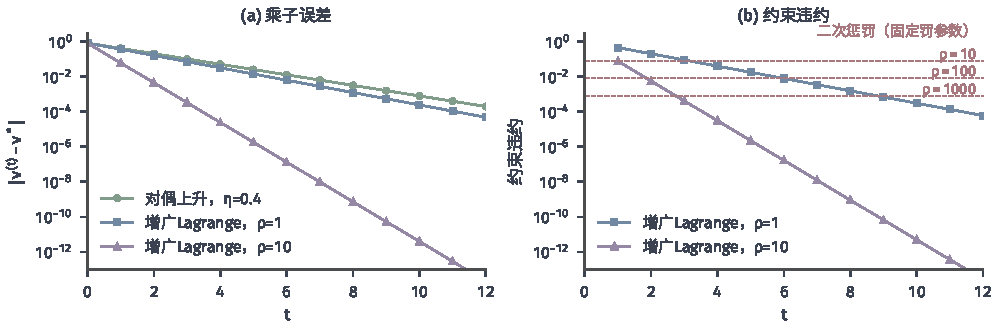
\includegraphics[width=169mm]{figures/03-optimization-evolution-and-signals/01-optimization/matplotlib/c5-al-multiplier/figure.pdf}
  \caption{等式二次例上的乘子更新，均从$\nu^{(0)}=0$出发，对数纵轴。(a) 乘子误差$|\nu^{(t)}-\nu^\star|$：对偶上升（$\eta=0.4$）每步减半；增广Lagrange法的收缩比率为$4/(4+5\rho)$，$\rho=1$时为$4/9$，$\rho=10$时约为$0.074$。(b) 内层点的约束违约：增广Lagrange法在固定$\rho$下持续下降；红色虚线是二次惩罚在$\rho=10,100,1000$时的违约$4/(4+5\rho)$，只能靠增大$\rho$减小。}
  \label{fig:opt-con-al-multiplier}
\end{figure*}

\paragraph{收敛条件与计算代价}
应分别追踪原始残差$\lVert\bm h(\bm x^{(t)})\rVert_2$、驻点残差（即内层容差）与内层求解精度。凸情形下，增广Lagrange法等价于对偶问题上的邻近点法（第~\ref{chap:opt-nonsmooth}章），在对偶最优解存在、内层精确求解时，对任意固定的$\rho>0$乘子都收敛；内层误差需要可求和地减小。一般非凸问题只有局部结论：在满足LICQ和二阶充分条件的局部解附近，$\rho$足够大且初始乘子足够接近时，算法局部收敛\scite{math-nocedal2006numerical}。$\rho$的选择仍是折中：较大的$\rho$让乘子收敛更快，但内层Hessian含$\rho\nabla\bm h^\top\nabla\bm h$，条件数随$\rho$增长，内层求解更难；与二次惩罚的区别在于$\rho$不必无限增大。不等式约束可以先引入松弛变量化为等式，再对松弛变量的非负性作投影。

本小节的内层仍把$\bm x$作为一个整体求解。平方项$\lVert\bm h(\bm x)\rVert_2^2$会把原本可分的变量耦合起来：即使$f$按块可分、约束是$\bm A\bm x+\bm B\bm z=\bm c$这样的线性耦合，$\lVert\bm A\bm x+\bm B\bm z-\bm c\rVert_2^2$也含交叉项，$\bm x$与$\bm z$不能再分开求解。下一小节正是为了恢复可分性而改变这一步。

\subsection{ADMM与一致性约束}
\label{sec:opt-con-admm}

\paragraph{两块交替的增广Lagrange步}
考虑两块可分的目标与线性耦合：
\[
  \min_{\bm x,\bm z}\ f(\bm x)+g(\bm z)\quad\text{s.t.}\quad\bm A\bm x+\bm B\bm z=\bm c.
\]
增广Lagrange函数为$\mathcal L_\rho(\bm x,\bm z,\bm\nu)=f(\bm x)+g(\bm z)+\bm\nu^\top(\bm A\bm x+\bm B\bm z-\bm c)+\frac\rho2\lVert\bm A\bm x+\bm B\bm z-\bm c\rVert_2^2$。增广Lagrange法需要对$(\bm x,\bm z)$联合最小化；\term{交替方向乘子法}（alternating direction method of multipliers，ADMM）只做一轮交替：先固定$\bm z$对$\bm x$最小化，再用新的$\bm x$对$\bm z$最小化，然后更新乘子。用缩放乘子$\bm u=\bm\nu/\rho$书写更简洁：

\begin{algorithm}[ADMM（缩放形式）]
\label{alg:opt-con-admm}
\begin{algorithmic}[1]
\Require $\bm z^{(0)}$、$\bm u^{(0)}$，罚参数$\rho>0$，容差$\epsilon_{\mathrm{pri}}$、$\epsilon_{\mathrm{dual}}$
\Ensure $(\bm x^{(t)},\bm z^{(t)},\rho\bm u^{(t)})$
\For{$t=0,1,2,\dots$}
  \State $\bm x^{(t+1)}=\argmin_{\bm x}\ f(\bm x)+\frac\rho2\lVert\bm A\bm x+\bm B\bm z^{(t)}-\bm c+\bm u^{(t)}\rVert_2^2$
  \State $\bm z^{(t+1)}=\argmin_{\bm z}\ g(\bm z)+\frac\rho2\lVert\bm A\bm x^{(t+1)}+\bm B\bm z-\bm c+\bm u^{(t)}\rVert_2^2$
  \State $\bm u^{(t+1)}=\bm u^{(t)}+\bm A\bm x^{(t+1)}+\bm B\bm z^{(t+1)}-\bm c$
  \State 原始残差$\bm r=\bm A\bm x^{(t+1)}+\bm B\bm z^{(t+1)}-\bm c$，对偶残差$\bm s=\rho\bm A^\top\bm B(\bm z^{(t+1)}-\bm z^{(t)})$；若$\lVert\bm r\rVert_2\leq\epsilon_{\mathrm{pri}}$且$\lVert\bm s\rVert_2\leq\epsilon_{\mathrm{dual}}$，停止
\EndFor
\end{algorithmic}
\end{algorithm}

$\bm x$步使用旧的$\bm z^{(t)}$，$\bm z$步使用刚算出的$\bm x^{(t+1)}$，次序不能对调成同时更新。对偶残差的形式来自$\bm z$步的最优性条件：精确的$\bm z$步使$(\bm x^{(t+1)},\bm z^{(t+1)},\bm\nu^{(t+1)})$满足关于$\bm z$的驻点条件，而关于$\bm x$的驻点条件恰好差$\bm s$。

\paragraph{分裂平方损失与正则项}
以$\ell_1$正则最小二乘为例：$f(\bm x)=\frac12\lVert\bm A\bm x-\bm b\rVert_2^2$、$g(\bm z)=\lambda\lVert\bm z\rVert_1$、约束$\bm x-\bm z=\bm0$。$\bm x$步是一个岭回归式的线性方程$(\bm A^\top\bm A+\rho\bm I)\bm x=\bm A^\top\bm b+\rho(\bm z^{(t)}-\bm u^{(t)})$，系数矩阵不随迭代变化，分解一次即可重复使用；$\bm z$步是第~\ref{chap:opt-nonsmooth}章的软阈值$\bm z=S_{\lambda/\rho}(\bm x^{(t+1)}+\bm u^{(t)})$。两个子问题各自只处理一种结构，这正是分裂的目的。

取最简单的标量情形$f(x)=\frac12(x-3)^2$、$g(z)=|z|$、约束$x=z$，最优解为软阈值$x^\star=z^\star=2$，最优乘子$\nu^\star=1$。取$\rho=1$，从$z=u=0$出发：$x$步$x=(3+z-u)/2=1.5$，$z$步$z=S_1(x+u)=0.5$，$u=u+x-z=1$；第二轮$x=(3+0.5-1)/2=1.25$，$z=S_1(2.25)=1.25$，$u=1$；第三轮$x=1.625$，$z=1.625$。此后$u$保持为$1=\nu^\star/\rho$，$x$与$z$相等，与$2$的距离每轮减半。图~\ref{fig:opt-con-admm}(a)在$(x,z)$平面上画出这条路径：$x$步沿水平方向移动，$z$步沿竖直方向移动，两种移动交替，逐渐收拢到约束线$x=z$上的最优点。图(b)比较不同$\rho$：在$u$稳定以后，本例的误差收缩比率为$\rho/(1+\rho)$，较小的$\rho$反而更快；一般问题中$\rho$同时影响原始残差与对偶残差的平衡，没有普遍最优的取值。

\begin{figure*}[!htbp]
  \centering
  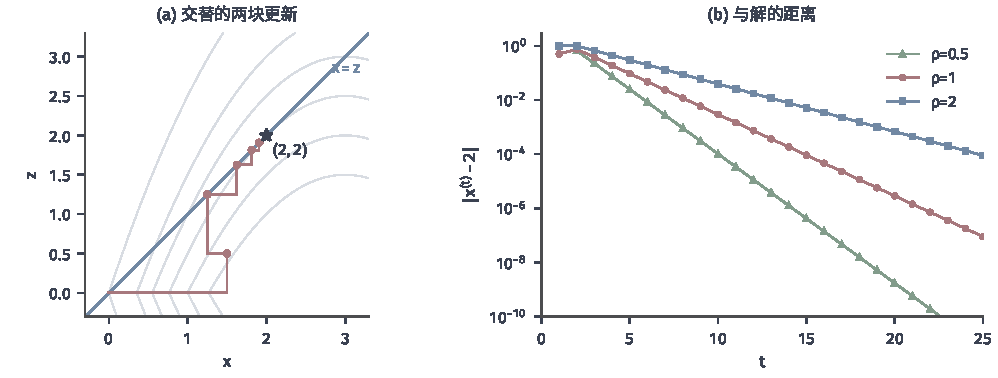
\includegraphics[width=169mm]{figures/03-optimization-evolution-and-signals/01-optimization/matplotlib/c5-admm/figure.pdf}
  \caption{标量问题$\min\frac12(x-3)^2+|z|$、$x=z$上的ADMM。(a) $\rho=1$，从$z=u=0$出发；灰色曲线为$\frac12(x-3)^2+|z|$的等值线，蓝线为约束$x=z$。红色折线中水平段是$x$步，竖直段是$z$步，红点为每轮结束时的$(x,z)$，收拢到五角星$(2,2)$。(b) 误差$|x^{(t)}-2|$（对数纵轴）在$\rho=0.5,1,2$下的变化；乘子稳定后误差按$\rho/(1+\rho)$收缩。本例中第二轮起$z^{(t)}=x^{(t)}$，原始残差恰为零。}
  \label{fig:opt-con-admm}
\end{figure*}

\paragraph{保证与适用范围}
ADMM的标准保证需要以下条件：$f,g$是闭适当凸函数；未增广的Lagrange函数$\mathcal L_0$有鞍点；两个子问题能精确求解（或误差可求和）。在这些条件下，原始残差$\bm r^{(t)}\to\bm0$，目标值$f(\bm x^{(t)})+g(\bm z^{(t)})\to f^\star$，乘子$\bm\nu^{(t)}$收敛到对偶最优解\scite{boyd2011admm}。注意这里没有断言$(\bm x^{(t)},\bm z^{(t)})$本身收敛；迭代点列的收敛需要额外条件（例如$\bm A,\bm B$列满秩），使用时要另行核查。收敛速度一般只是次线性的，适合中等精度的求解。

ADMM最适合一致性形式的问题：$\min\sum_{k=1}^Kf_k(\bm x_k)+g(\bm z)$、$\bm x_k=\bm z$。$\bm x$步对各$k$完全分离，可以在$K$台机器上并行；每轮通信只需收集$\bm x_k+\bm u_k$，在中心求$\bm z$（$g=0$时就是取平均），再广播回去。与对偶分解相比，它的每个子问题都含平方项，对仅凸的$f_k$也有良好定义，代价是子问题多了一个二次项。直接把两块的交替推广到三块或更多块，即使问题凸，也可能发散\scite{chen2016admm}；非凸问题中的ADMM也没有同样的保证，需要针对具体结构另作分析。
